\documentclass{beamer}

\usecolortheme[dark,accent=cyan]{solarized}

\beamertemplatenavigationsymbolsempty

\usepackage{coloremoji}
\usepackage{graphicx}
\usepackage{hyperref}
\usepackage{colortbl, xcolor}
\usepackage{booktabs}
\usepackage{varwidth}
\usepackage{hyperref}

\usepackage{tikz}
\usetikzlibrary{positioning,calc}
\usetikzlibrary{automata}
\usepackage{pstricks}
\usepackage{minted}

\definecolor{DarkGray}{gray}{0.1}
\definecolor{DarkGray}{gray}{0.1}
\usemintedstyle{native}

\begin{document}

\begin{frame}[fragile]
    \centering
        \textbf{\textcolor{orange}{\scriptsize{https://nikoleta-v3.github.io/blog/2018/01/24/choose-reviewers.html}}}
        \vspace{.3cm}
\begin{columns}
    \begin{column}{.65\linewidth}
    \begin{minted}
    [
    framesep=4mm,
    baselinestretch=1.2,
    bgcolor=DarkGray,
    fontsize=\tiny,
    ]
    {python}
>>> keywords = ['keyword one', 'keyword two', 
                'keyword three']
>>> def find_reviewers(names, keywords):
...    authors_of_interest = []
...    for name in names:
...         df = read_author_files(name)
...         for key in keywords:
...             if check_keyword_in_abstract(key, df):
...                 authors_of_interest.append((name, key))
...    return authors_of_interest
>>> find_reviewers(names, keywords)
    \end{minted}
    \end{column}
    \begin{column}{.26\linewidth}

    \end{column}
    \end{columns}
    \begin{columns}
        \begin{column}{.26\linewidth}
        \end{column}
    \begin{column}{.65\linewidth}
        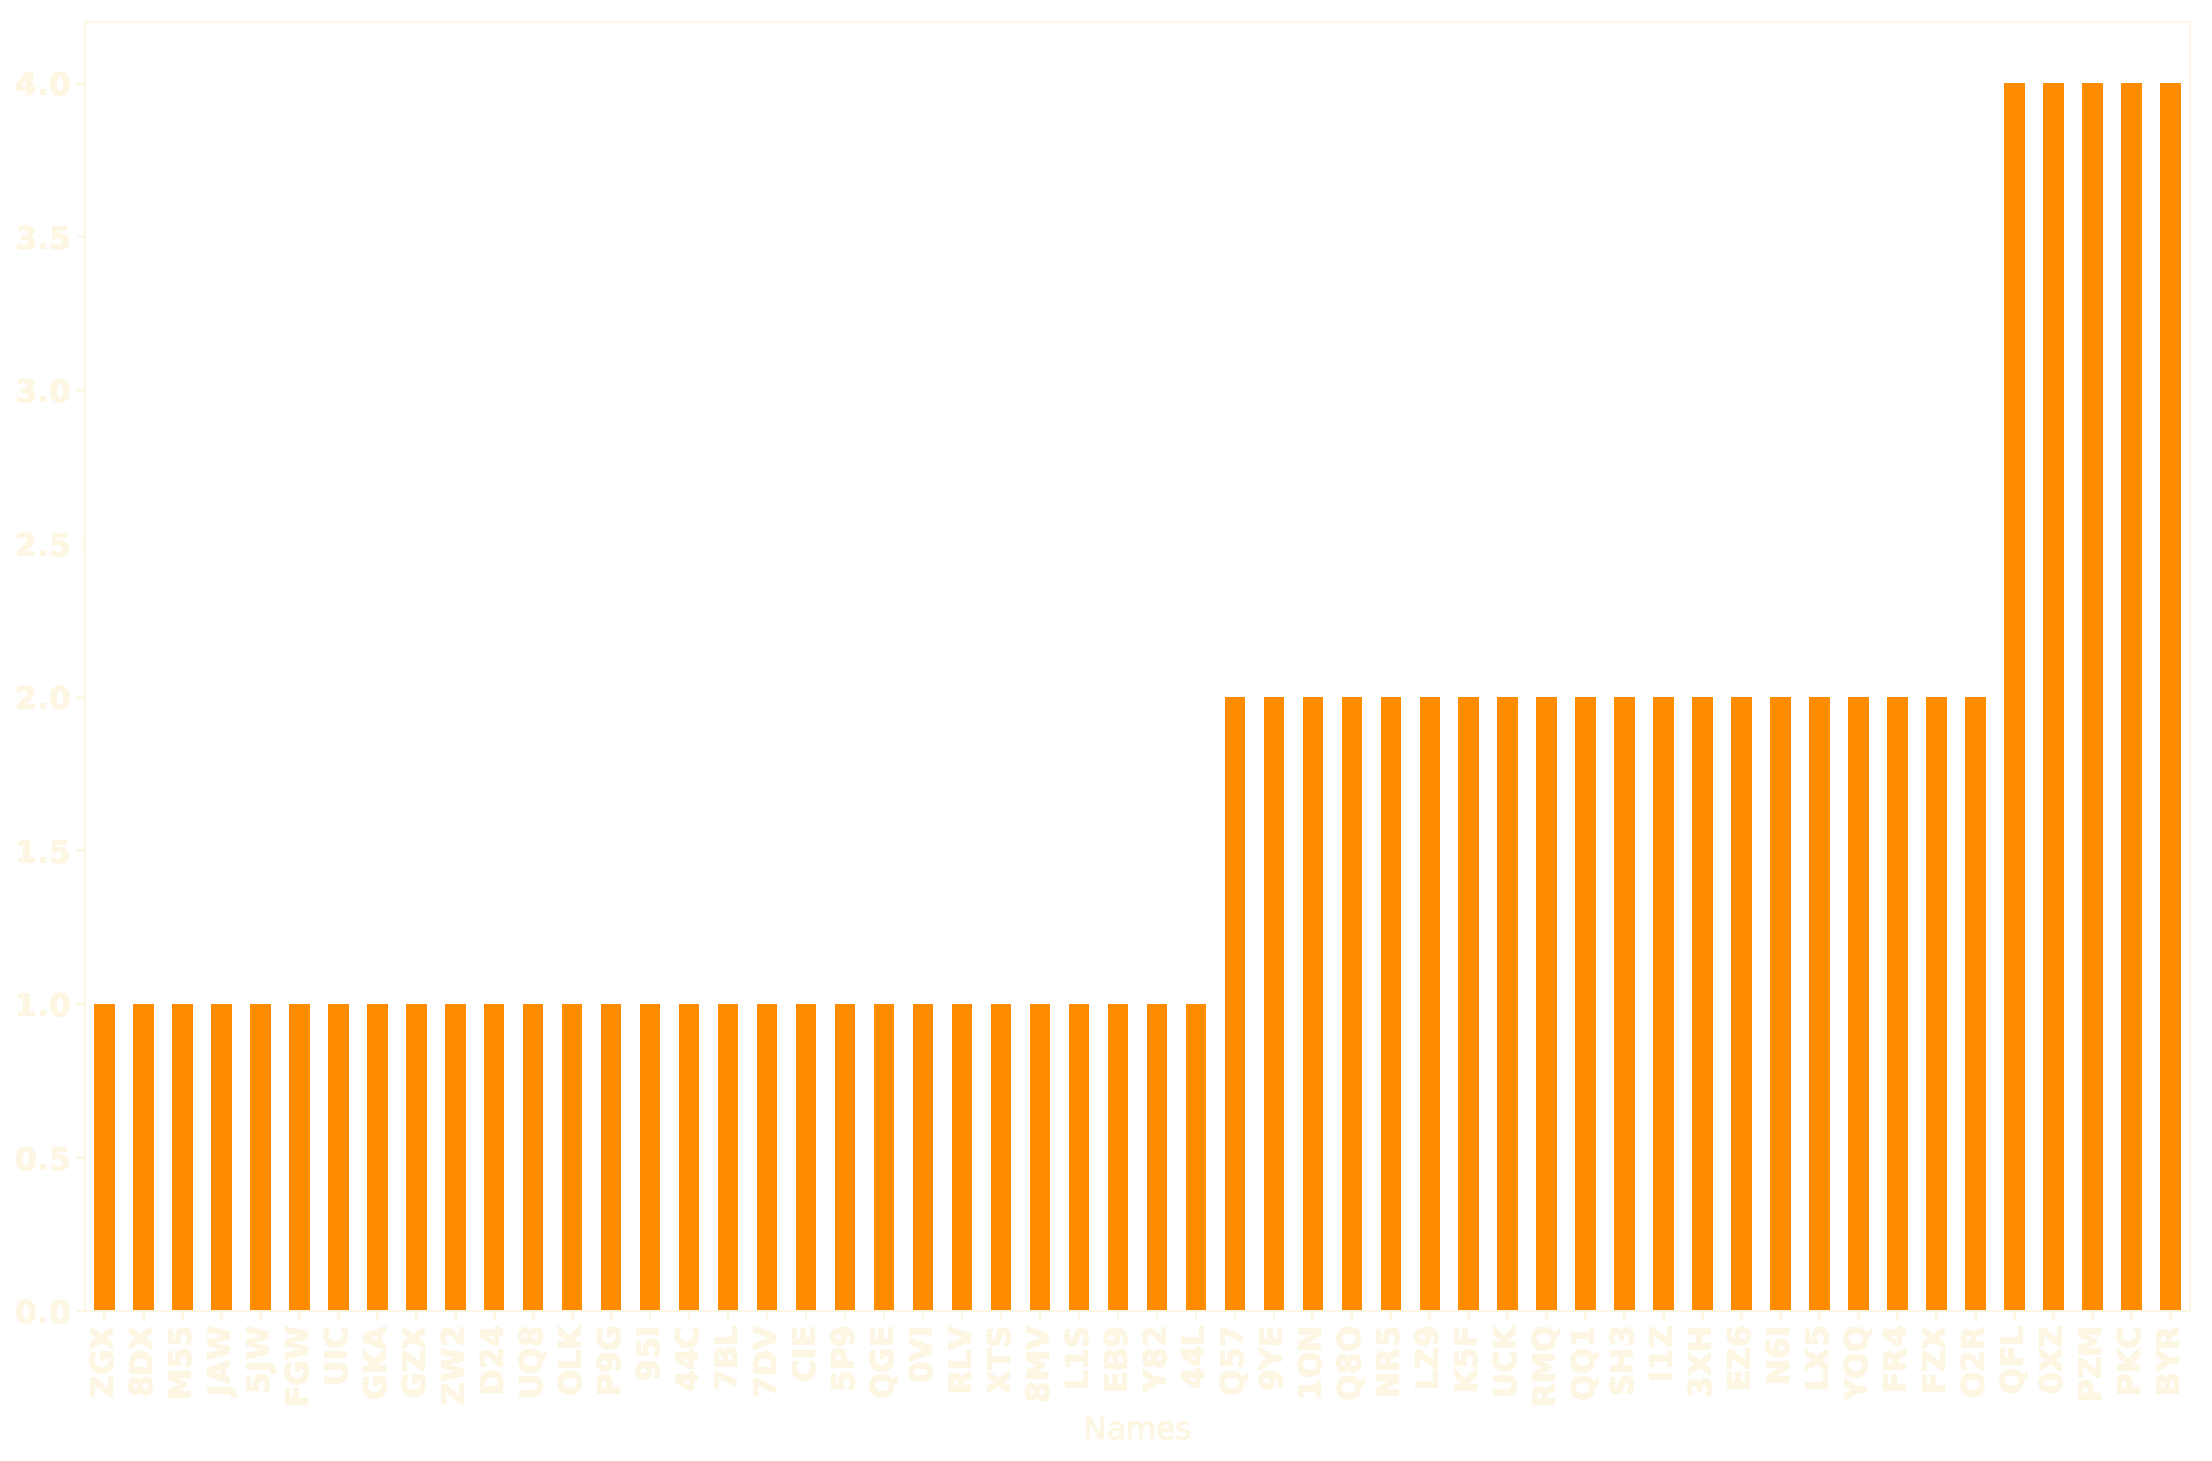
\includegraphics[width=\textwidth, height=.42\textheight]{reviewers_hist.pdf}
    \end{column}
    \end{columns}
    \begin{minted}
        [
        framesep=2mm,
        baselinestretch=1.2,
        bgcolor=DarkGray,
        fontsize=\tiny,
        ]
        {python}
$ pip install arcas                 $ pip install pandas               $ pip install matplotlib
    \end{minted}
\end{frame}
\end{document}




